% chapter09.tex

 %%%%%%%%%%%%%%%%%%%%%%%%%%%%%%%%%%%%%%%%%%%%%%%%%%%%%%%%%%%%%%%%%%%%%%%%%%%%%
 %                                                                           %
 %    PyMS documentation                                                     %
 %    Copyright (C) 2005-8 Vladimir Likic                                    %
 %                                                                           %
 %    The files in this directory provided under the Creative Commons        %
 %    Attribution-NonCommercial-NoDerivs 2.1 Australia license               %
 %    http://creativecommons.org/licenses/by-nc-nd/2.1/au/                   %
 %    See the file license.txt                                               %
 %                                                                           %
 %%%%%%%%%%%%%%%%%%%%%%%%%%%%%%%%%%%%%%%%%%%%%%%%%%%%%%%%%%%%%%%%%%%%%%%%%%%%%

\chapter{GCMS Simulator}

The PyMS GCMS data simulator is a useful tool for creating datasets with known
peaks. 



\section{Setting up input data for the simulator}

The PyMS GCMS data simulator package provides an Intensity Matrix object 
which can be processed by PyMS in 
the same way as any Intensity Matrix object derived from real data.

As input, the simulator requires a list of peaks, a list of times and a list of
m/z channels. In this example we will use the time list, mass list and PyMS detected
peak list from an existing real GCMS dataset.

For the purpose of demonstrating the simulator, only a portion of this dataset is 
examined. The following code selects the area of interest in the dataset and
limits subsequent processing to this interval:

\begin{verbatim}
... data is a GCMS data object
>>> data.trim(4101, 4350)
\end{verbatim}

\subsection{Providing input to the simulator}
\noindent
[ {\em This example is in pyms-test/90} ]

The peaks are detected using the PyMS function {\tt BillerBiemann()}, and subsequently
filtered to remove those which do not meet certain requirements. This procedure is
fully detailed in section \ref{sec:peak-detection}.

Next the time list and mass list of the original data are copied to be used in the
simulator 
\begin{verbatim}
>>> mass_list = real_im.get_mass_list()
>>> time_list = real_im.get_time_list()
\end{verbatim}

, where {\tt real\_im} is the Intensity Matrix object derived from the real data. (For
more information about Intensity Matrix and data conversion refer to section (
\ref{sec:intensity-matrix}).

\section{Running the simulator}
The function {\tt gcms\_sim()} takes three inputs: time list, mass list and peak list.
It returns an Intensity Matrix object which can be manipulated in PyMS.

\begin{verbatim}
>>> sim_im = gcms_sim(time_list, mass_list, peak_list)
\end{verbatim}

Using the PyMS display functionality described in chapter \ref{chapter:display}, the results of 
the simulator can be viewed. Figure \ref{fig:no-noise} shows the IonChromatograms of the 
simulated Intensity Matrix.

\begin{figure}[h]
  \begin{center}
    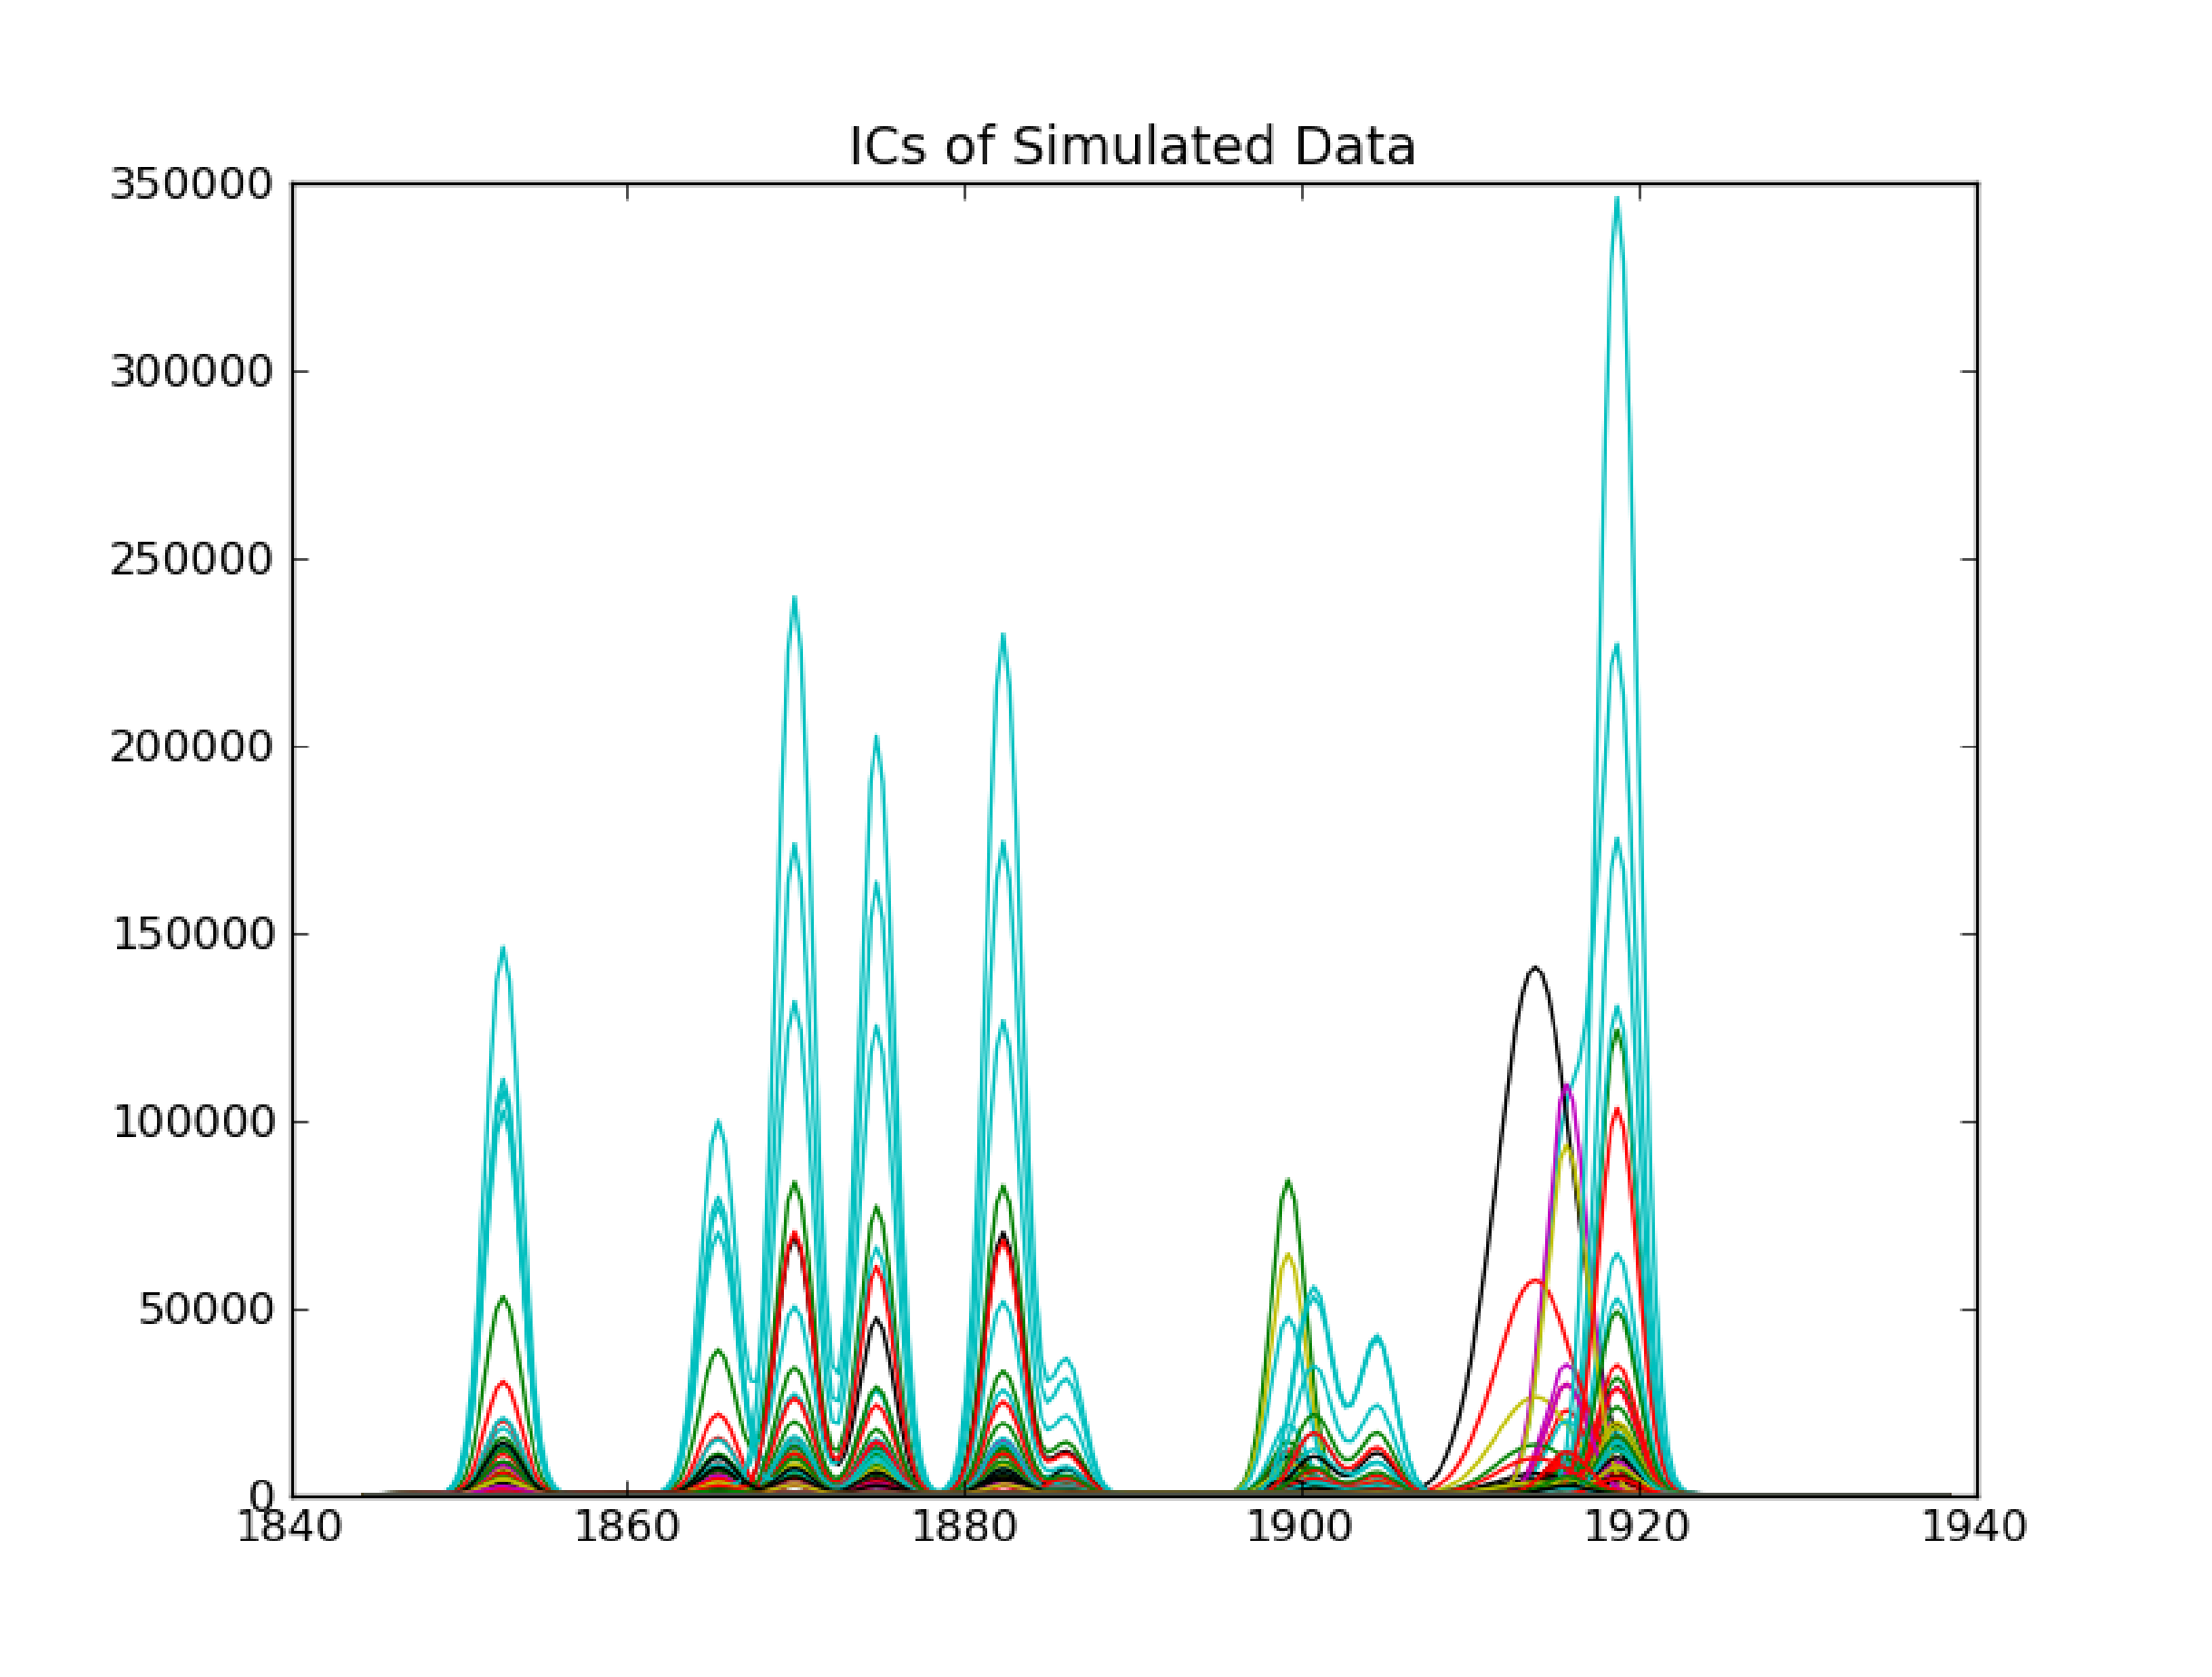
\includegraphics[scale=0.25]{graphics/chapter10/test-100.eps}
  \end{center}
  \caption{Graphics window displayed by the script 100/proc.py}
  \label{fig:no-noise}
\end{figure}

\section{Adding noise to the simulated data}
Noise can be added to either the full Intenstity Matrix, or to individual
Ion Chromatograms. Currently two noise models have been implemented in PyMS. 
These are:

\begin{enumerate}
  \item Gaussian noise drawn from a normal distribution with constant scale across all scans.
  \item Gaussian noise drawn from a normal distribution with scale varying with the intensity
value at that point.
\end{enumerate}


\subsection{Constant scale noise}

\noindent
[ {\em This example is in pyms-test/91} ]

The Python package NumPy contains routines for pseudo random number generation. These
"random" values are drawn from a normal distribution with a user defined scale over the same number
of samples as the number of scans in a GC-MS experiment. This resulting list of numbers is a 
good approximation to gaussian noise on an m/z channel in the GC-MS experiment. 

To add gaussian noise to an IC, the following code is used:

\begin{verbatim}
>>> ic = sim_im.get_ic_at_mass(73)
>>> scale = 1000
>>> add_gaussc_noise_ic(ic, scale)
\end{verbatim}

The normal distribution from which the noise values are drawn in this example has a top value of 1000.
This noisy IC can be displayed using the PyMS package Display, the resulting figure is shown in figure
\ref{fig:gaussc-noise-ic}.

\begin{figure}[h]
  \begin{center}
    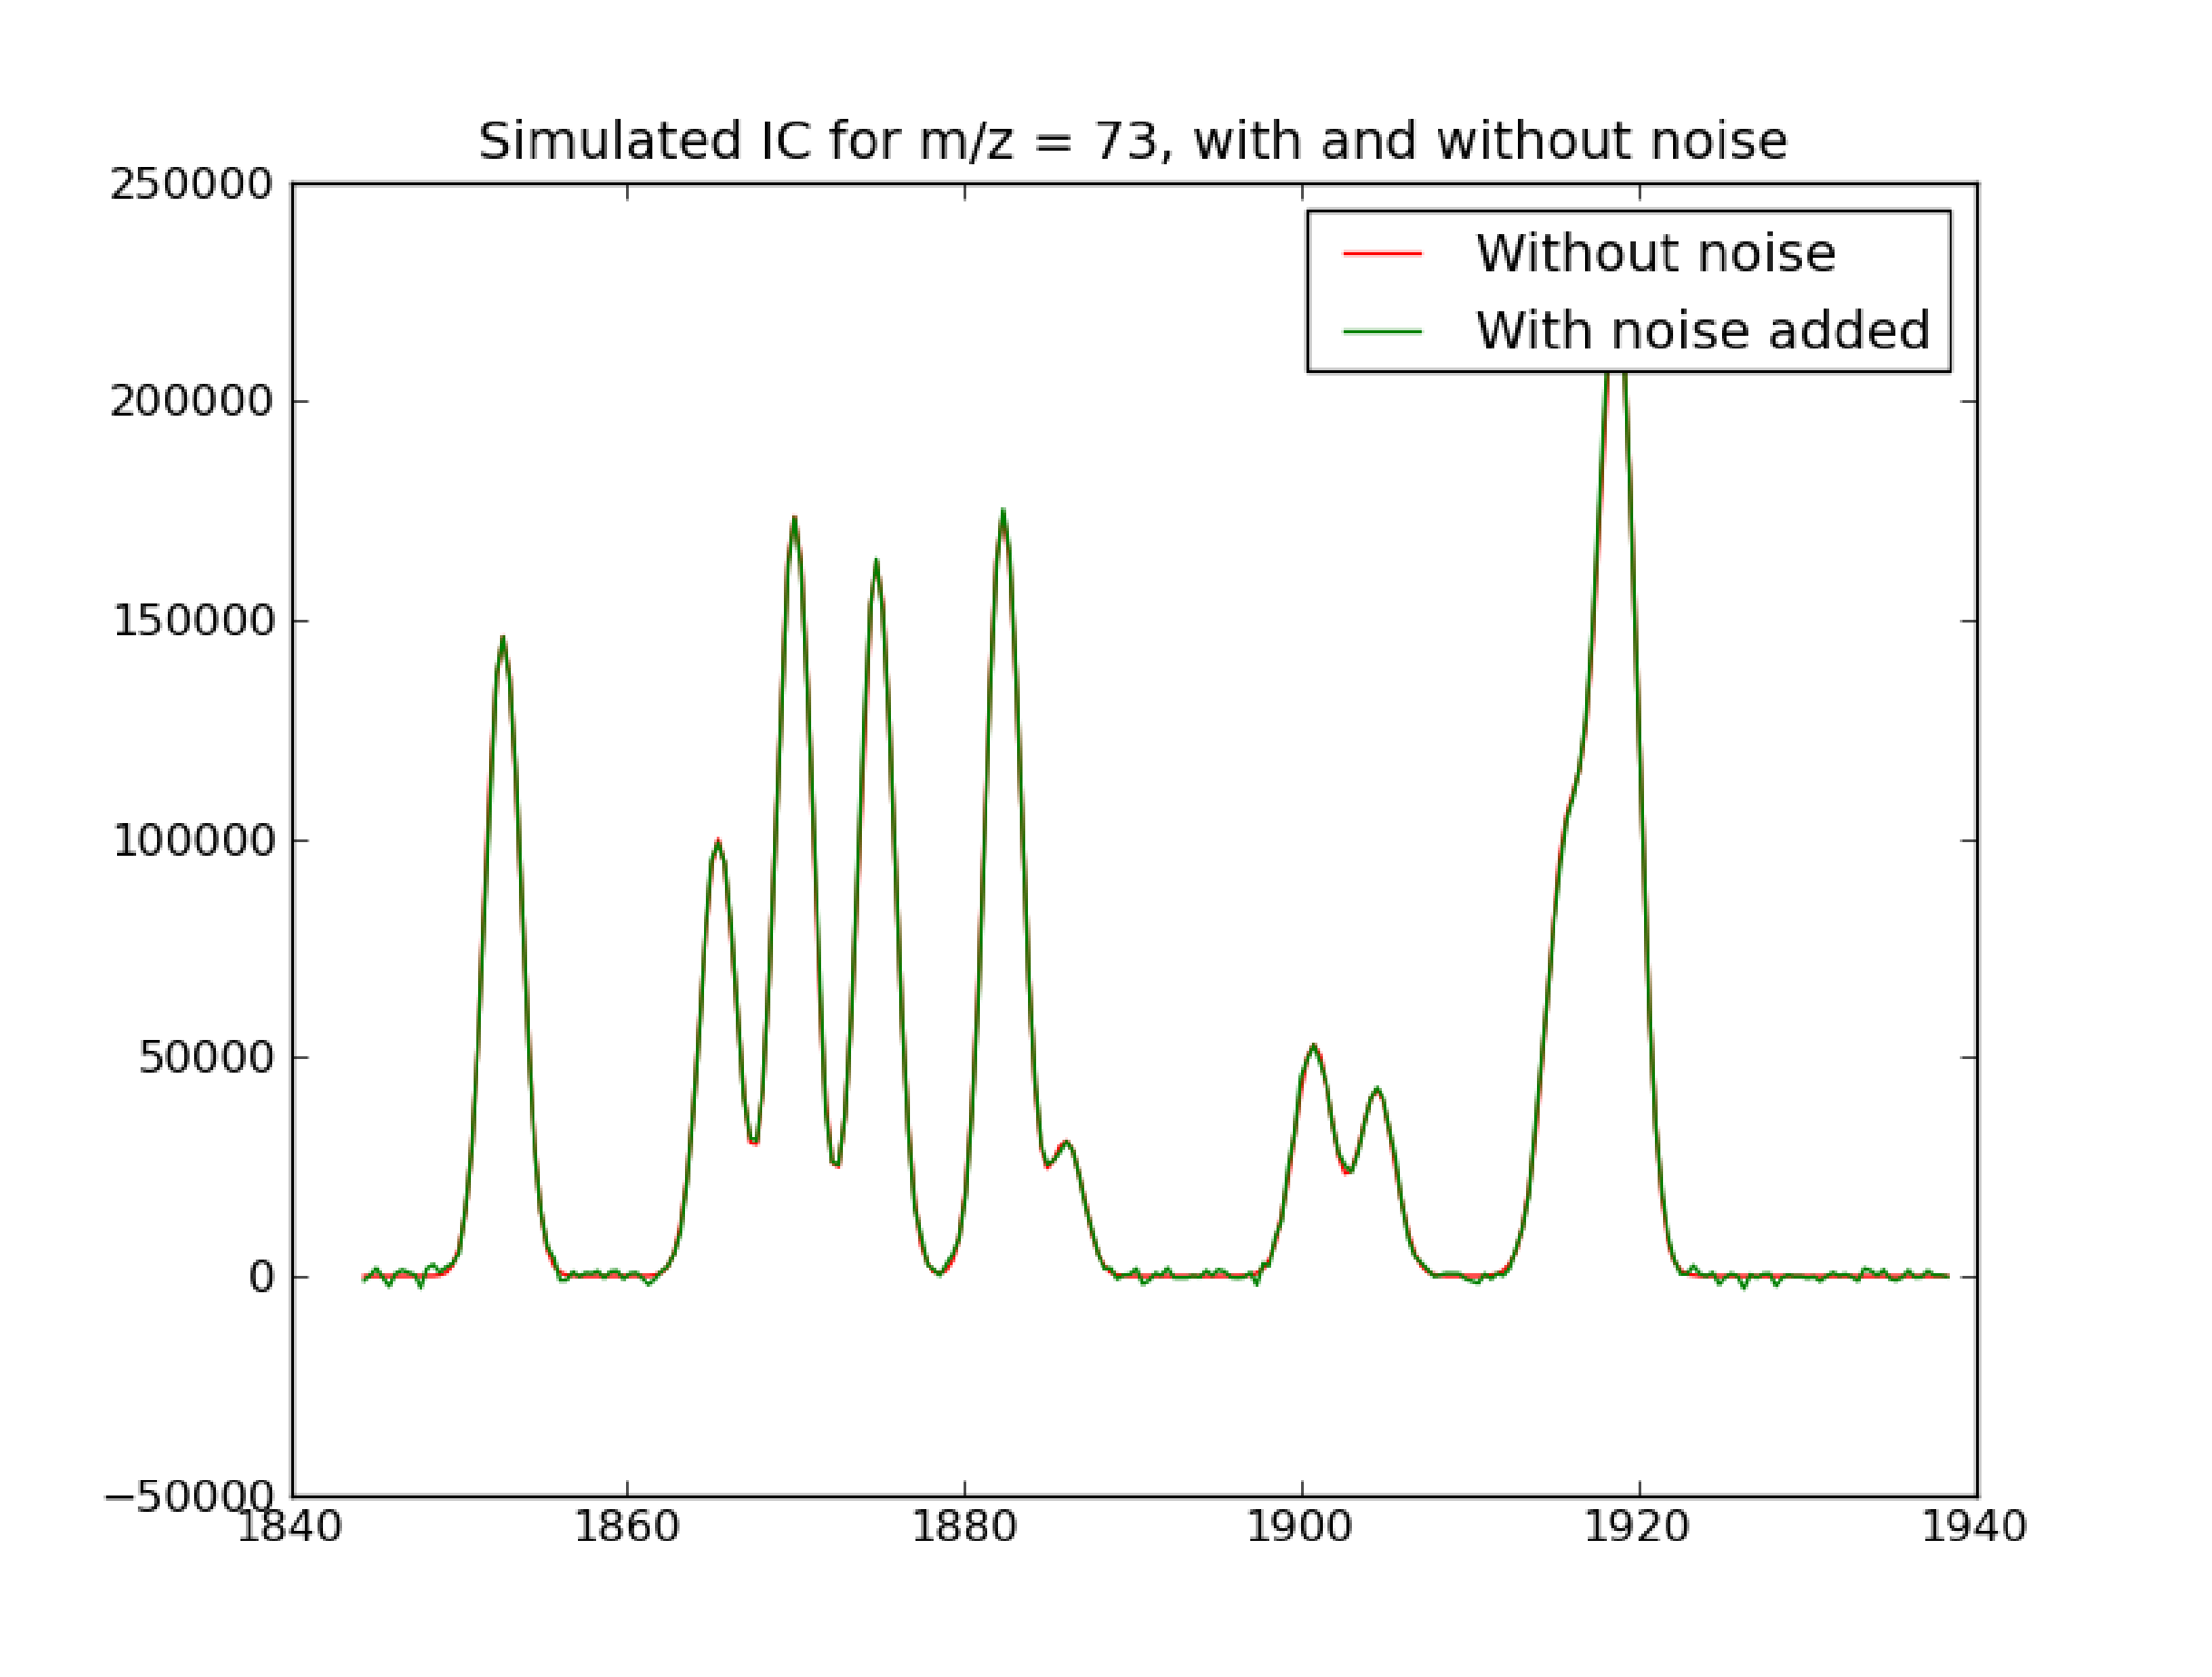
\includegraphics[scale=0.25]{graphics/chapter09/test-91.eps}
  \end{center}
  \caption{Graphics window displayed by the script 91/proc.py}
  \label{fig:gaussc-noise-ic}
\end{figure}


\subsection{Variable scale noise}
\label{subsec:gaussv-noise-ic}

\noindent
[ {\em This example is in pyms-test/92} ]

In reality, noise from a GC-MS experiment tends to have higher values in areas where peaks occur than in
the valleys between peaks. To attempt to model this, a variable scale noise function has been implemented in
PyMS. For a given time-point in an Ion Chromatogram, if the intensity at that time-point is greater than
a user defined threshold value, the scale of the normal distribution from which the noise value is drawn will be 
proportional to the intensity at that point. The actual scale of the distribution at that point will be
{\tt scale * (intensity*proportion)}, if the intensity is above the {\tt cutoff} value, and {\tt scale} if below.

To add variable scale gaussian noise to an IC, the following code is used:

\begin{verbatim}
>>> ic = sim_im.get_ic_at_mass(73)
>>> scale = 1000
>>> cutoff = 10000
>>> prop = 0.0003
>>> add_gaussv_noise_ic(ic, scale, cutoff, prop)
\end{verbatim}

The resulting noisy IC is shown in figure \ref{fig:gaussv-noise-ic}


\begin{figure}[h]
  \begin{center}
    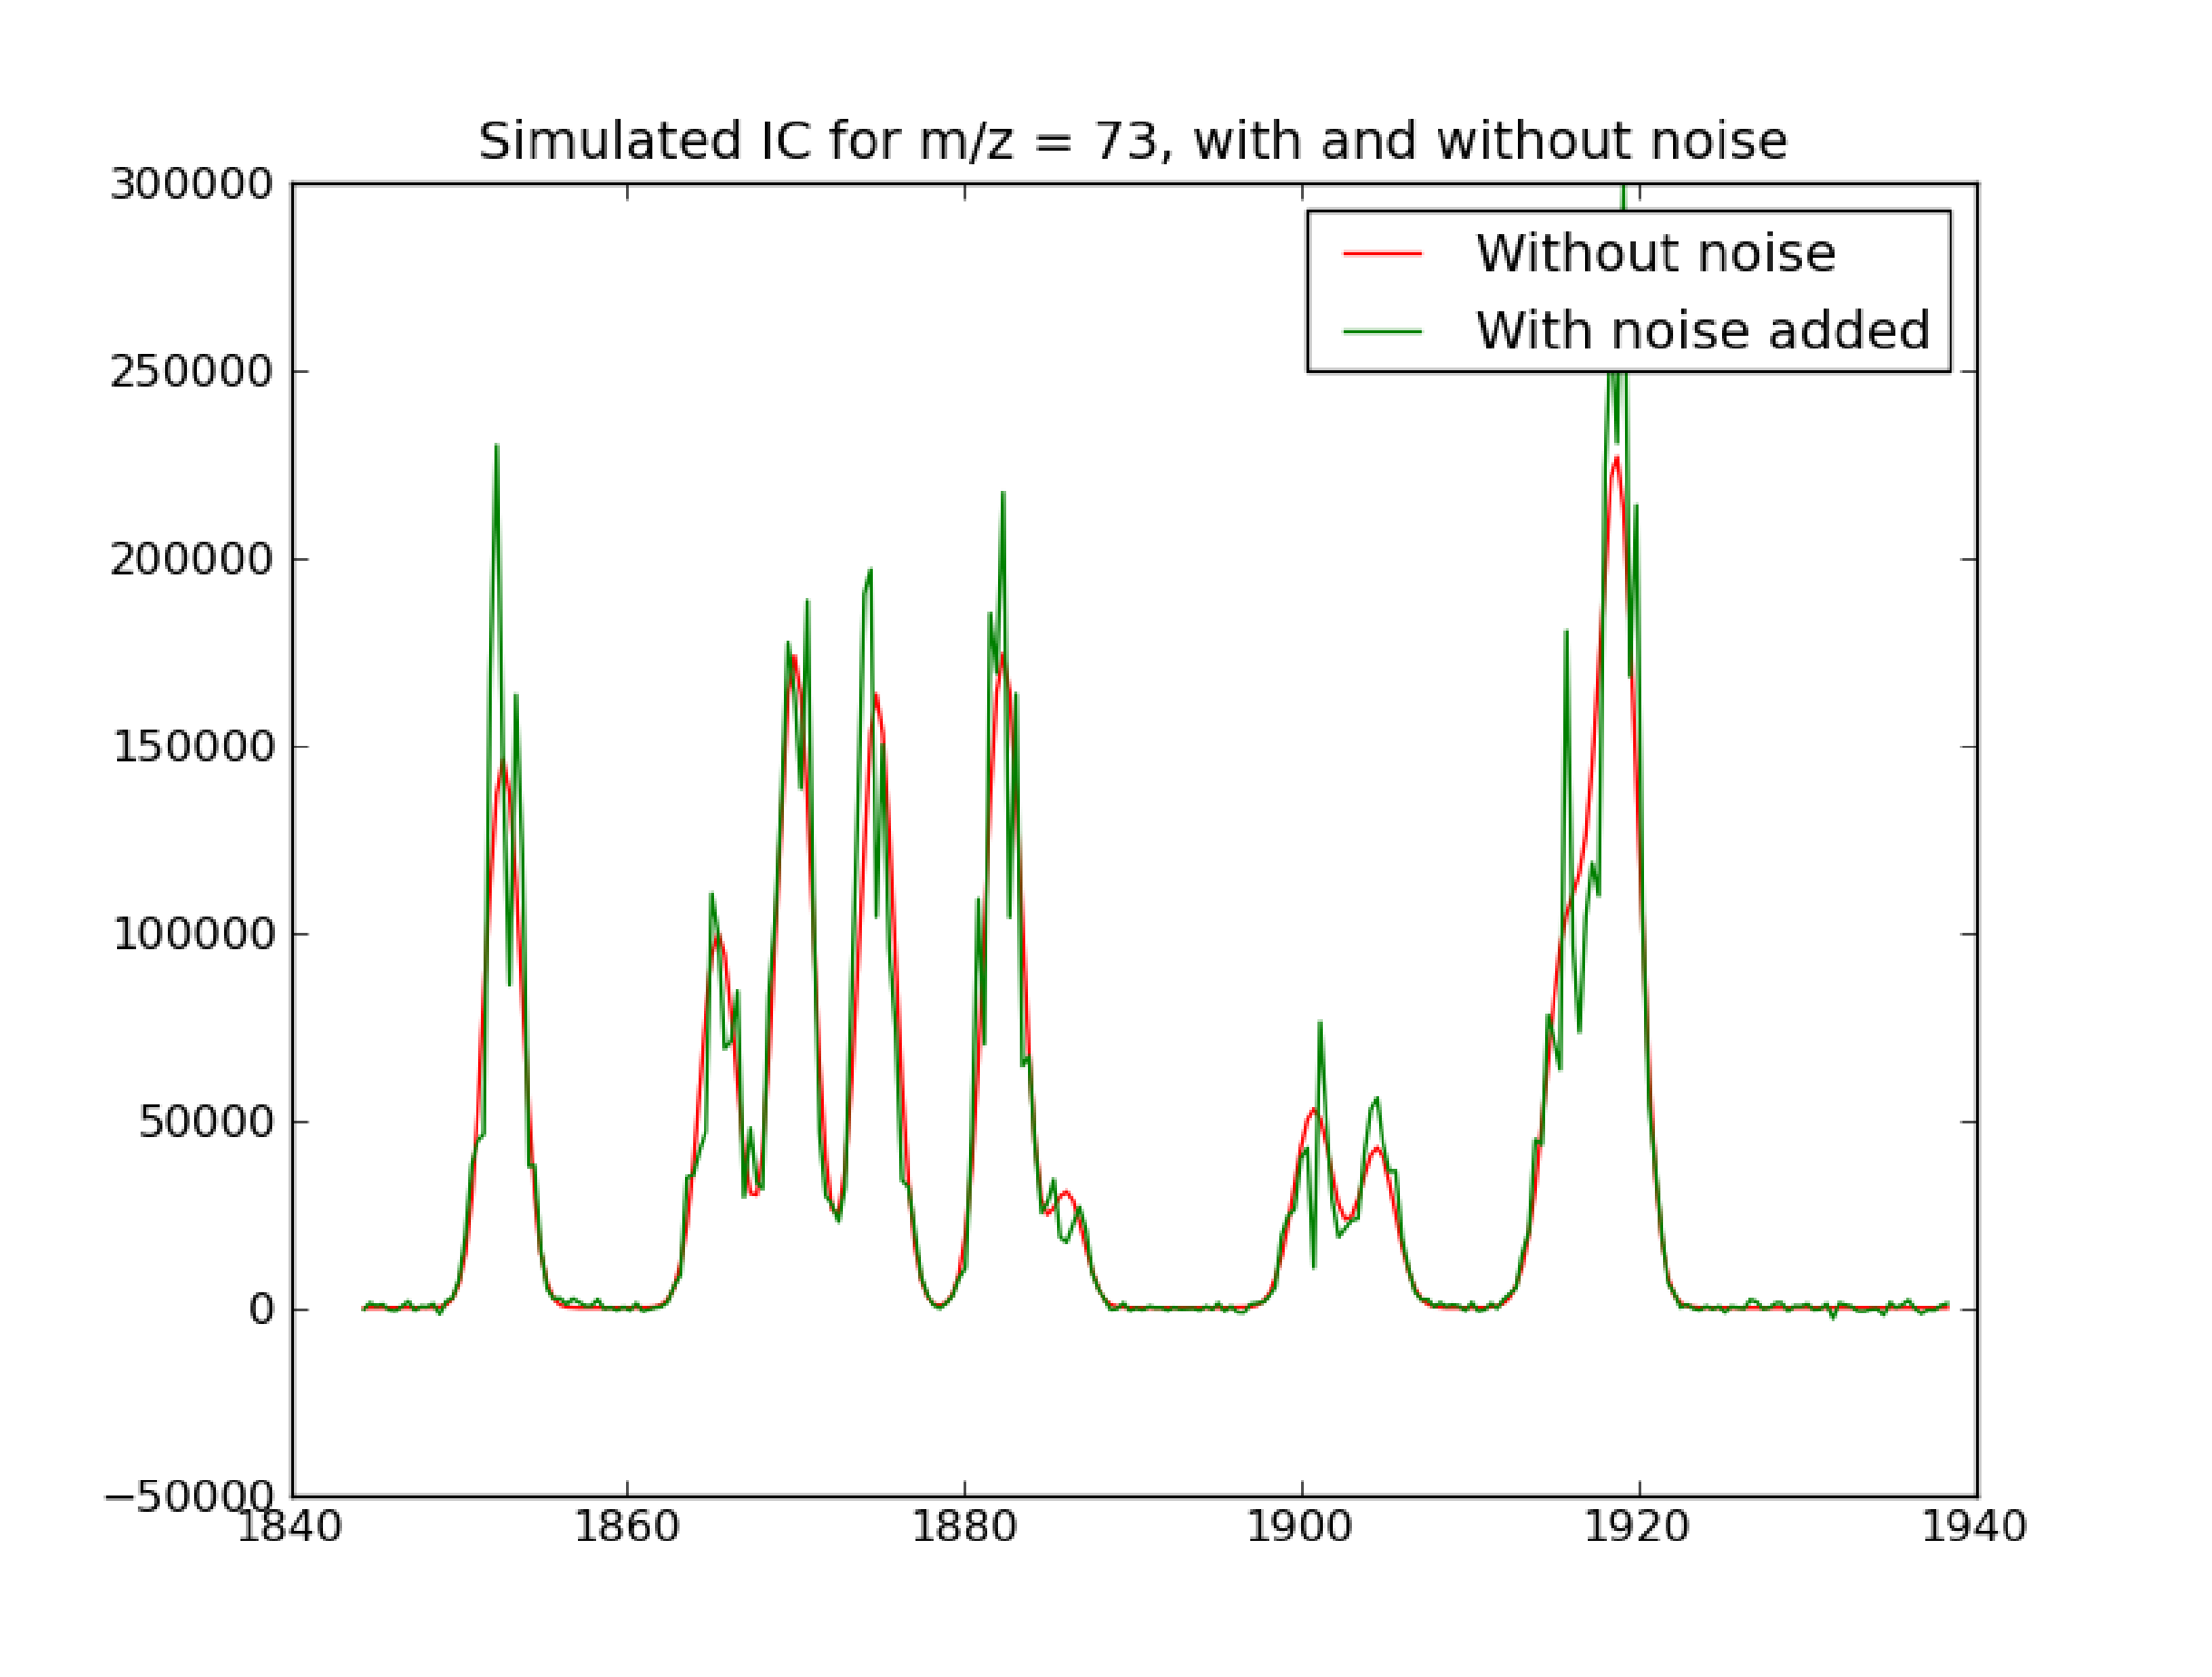
\includegraphics[scale=0.25]{graphics/chapter09/test-92.eps}
  \end{center}
  \caption{Graphics window displayed by the script 92/proc.py}
  \label{fig:gaussv-noise-ic}
\end{figure}



\section{{Adding noise to the whole simulated dataset}}


Often, the user may desire to add noise to all ICs in the dataset. This can be 
accomplished easily using the functions {\tt add\_gaussc\_noise()} and {\tt add\_gaussv\_noise()}
The noise models in question are exactly the same as for the single IC noise functions above.

\subsection{Constant scale gaussian noise}

\noindent
[ {\em This example is in pyms-test/93} ]
For constant scale gaussian noise:

\begin{verbatim}
... sim_im is a simulated intensity matrix object
>>> scale = 1000
>>> add_gaussc_noise(sim_im, scale)
\end{verbatim}

This code adds noise to all Ion Chromatograms in the Intensity Matrix. These can be 
viewed in the PyMS package Display, with the resulting figure shown below (figure 
\ref{fig:gaussc-noise}).



\begin{figure}[h]
  \begin{center}
    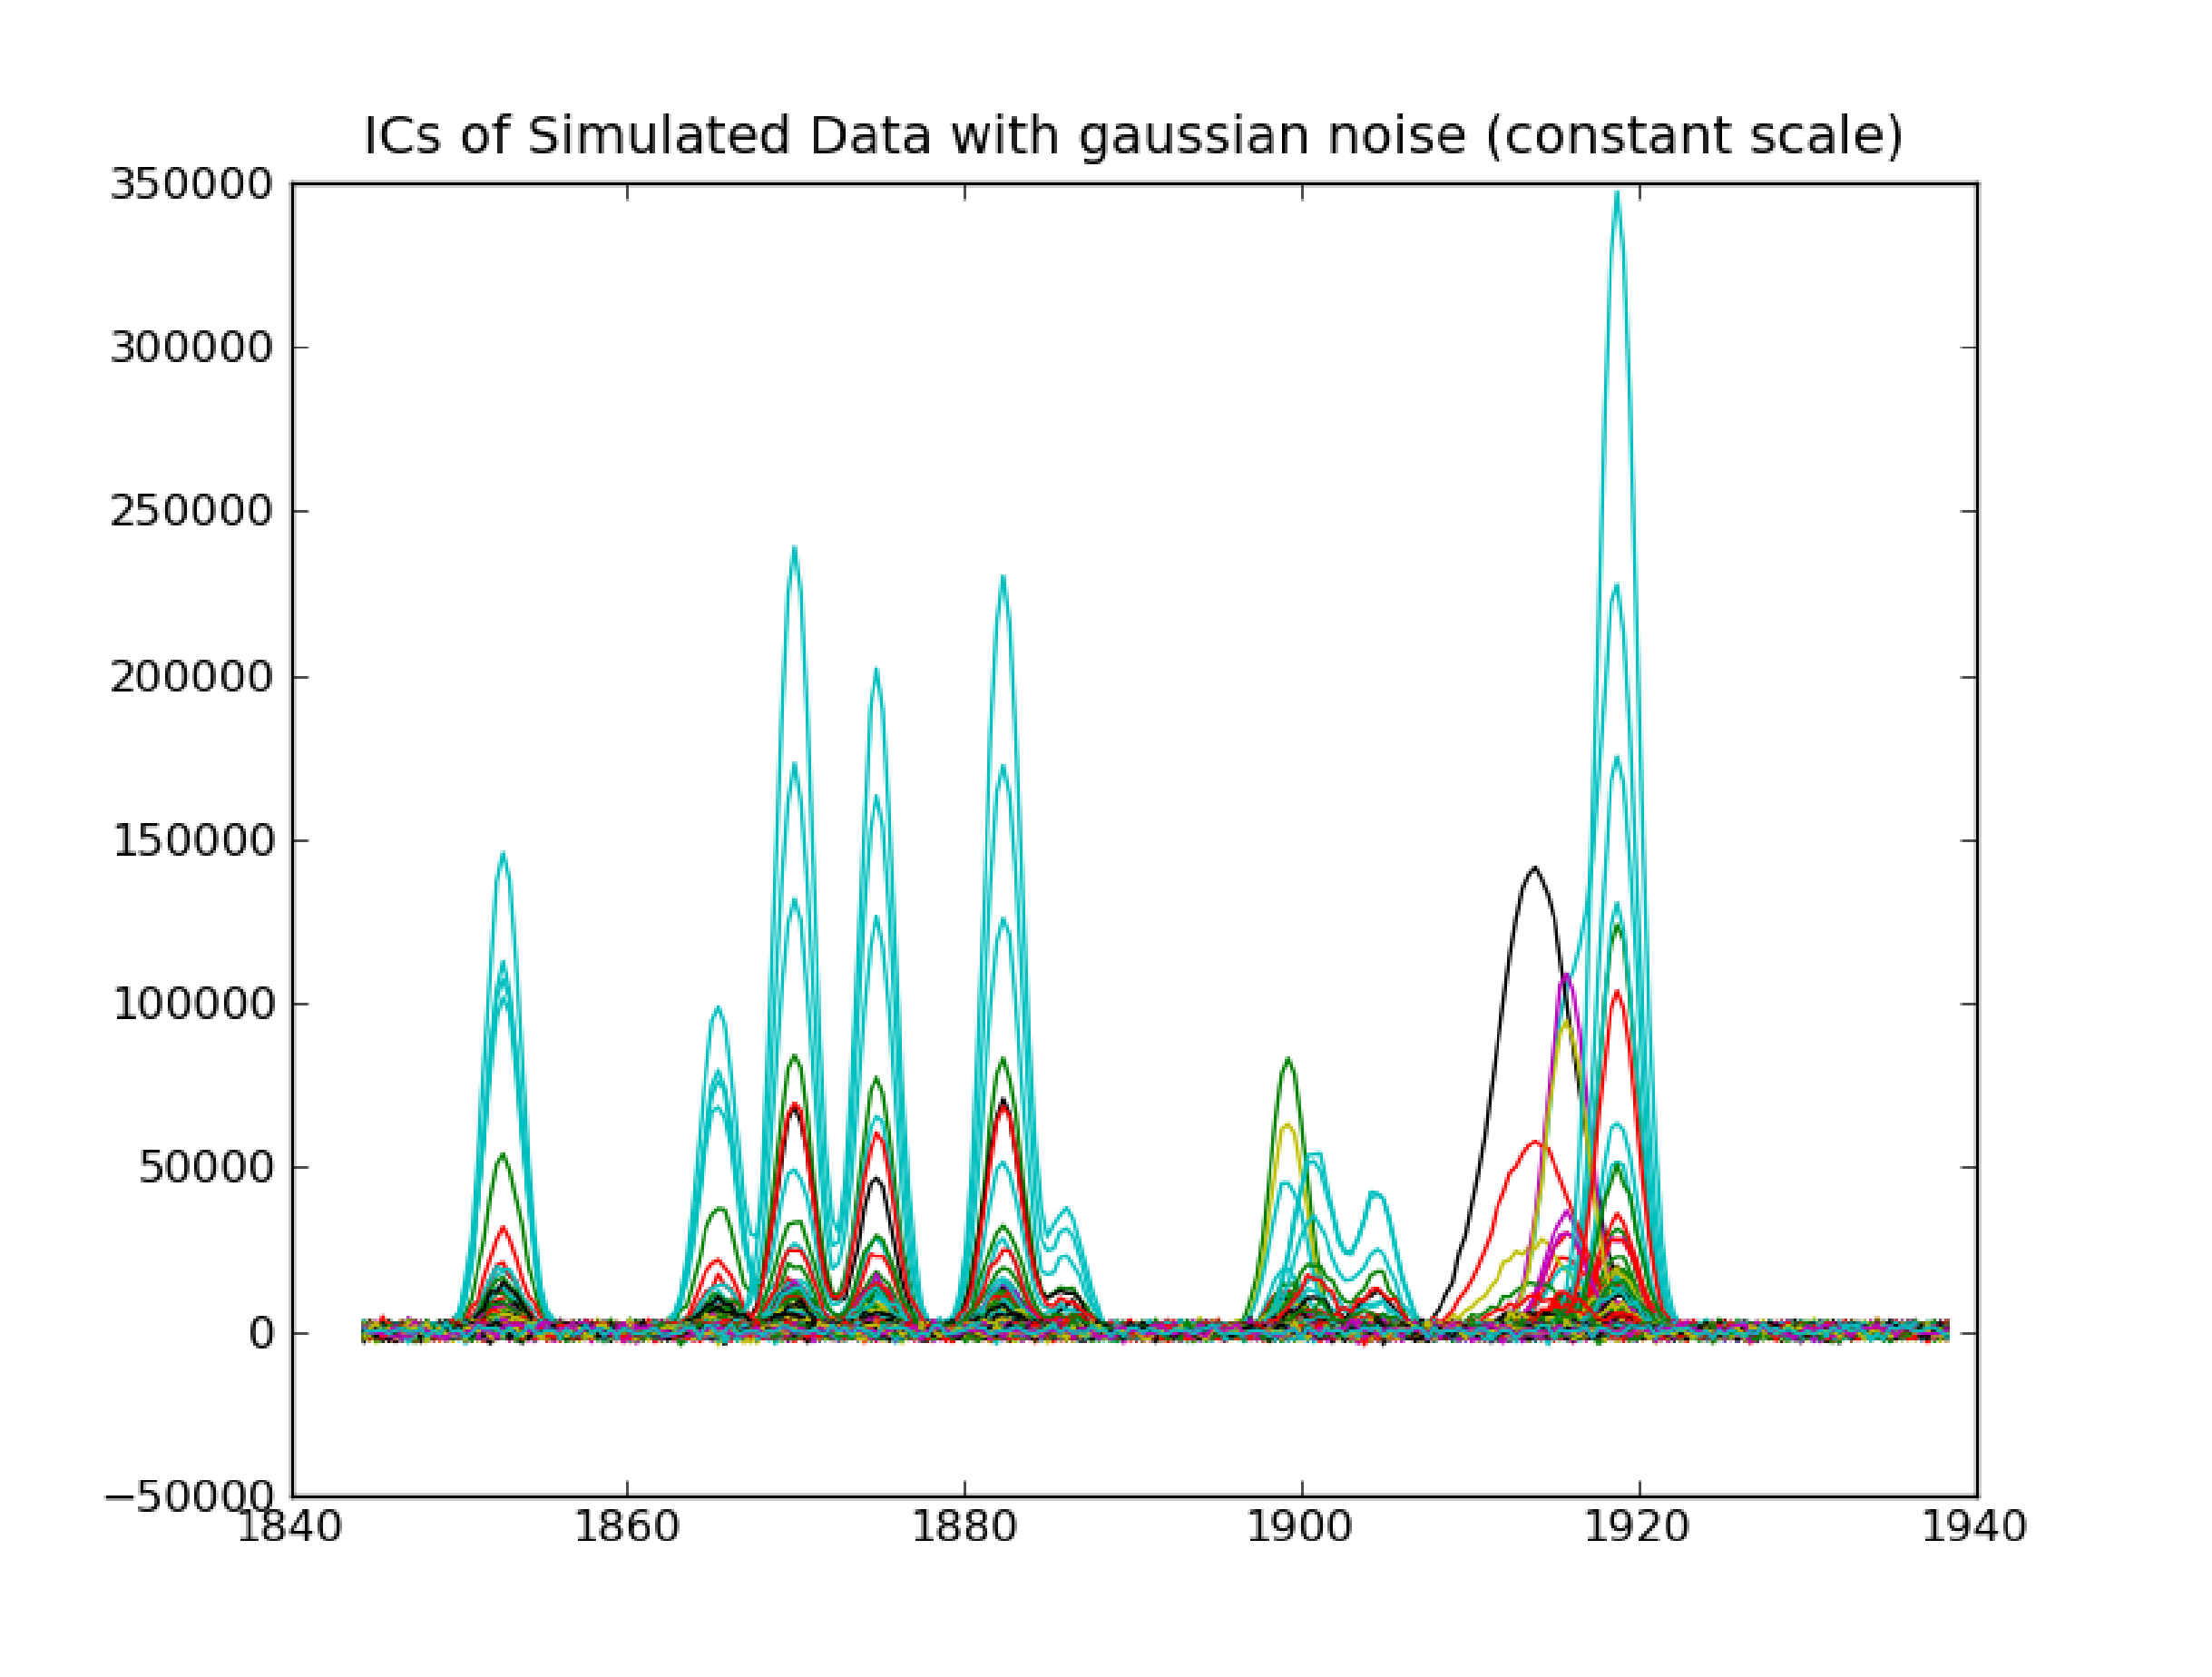
\includegraphics[scale=0.25]{graphics/chapter09/test-93.eps}
  \end{center}
  \caption{Graphics window displayed by the script 103/proc.py}
  \label{fig:gaussc-noise}
\end{figure}


\subsection{Variable scale gaussian noise}
\label{subsec:gaussv-noise}
\noindent
[ {\em This example is in pyms-test/94} ]

To apply variable scale gaussian noise to the whole simulated dataset:

\begin{verbatim}
>>> scale = 1000
>>> cutoff = 10000
>>> prop = 0.0003
>>> add_gaussv_noise(sim_im, scale, cutoff, prop)
\end{verbatim}

The arguments supplied to {\tt add\_gaussv\_noise()} relate to how the gaussian distribution
supplying the noise values changes with the intensity. These parameters are further discussed in 
sub-section \ref{subsec:gaussv-noise-ic} above.

\begin{figure}[h]
  \begin{center}
    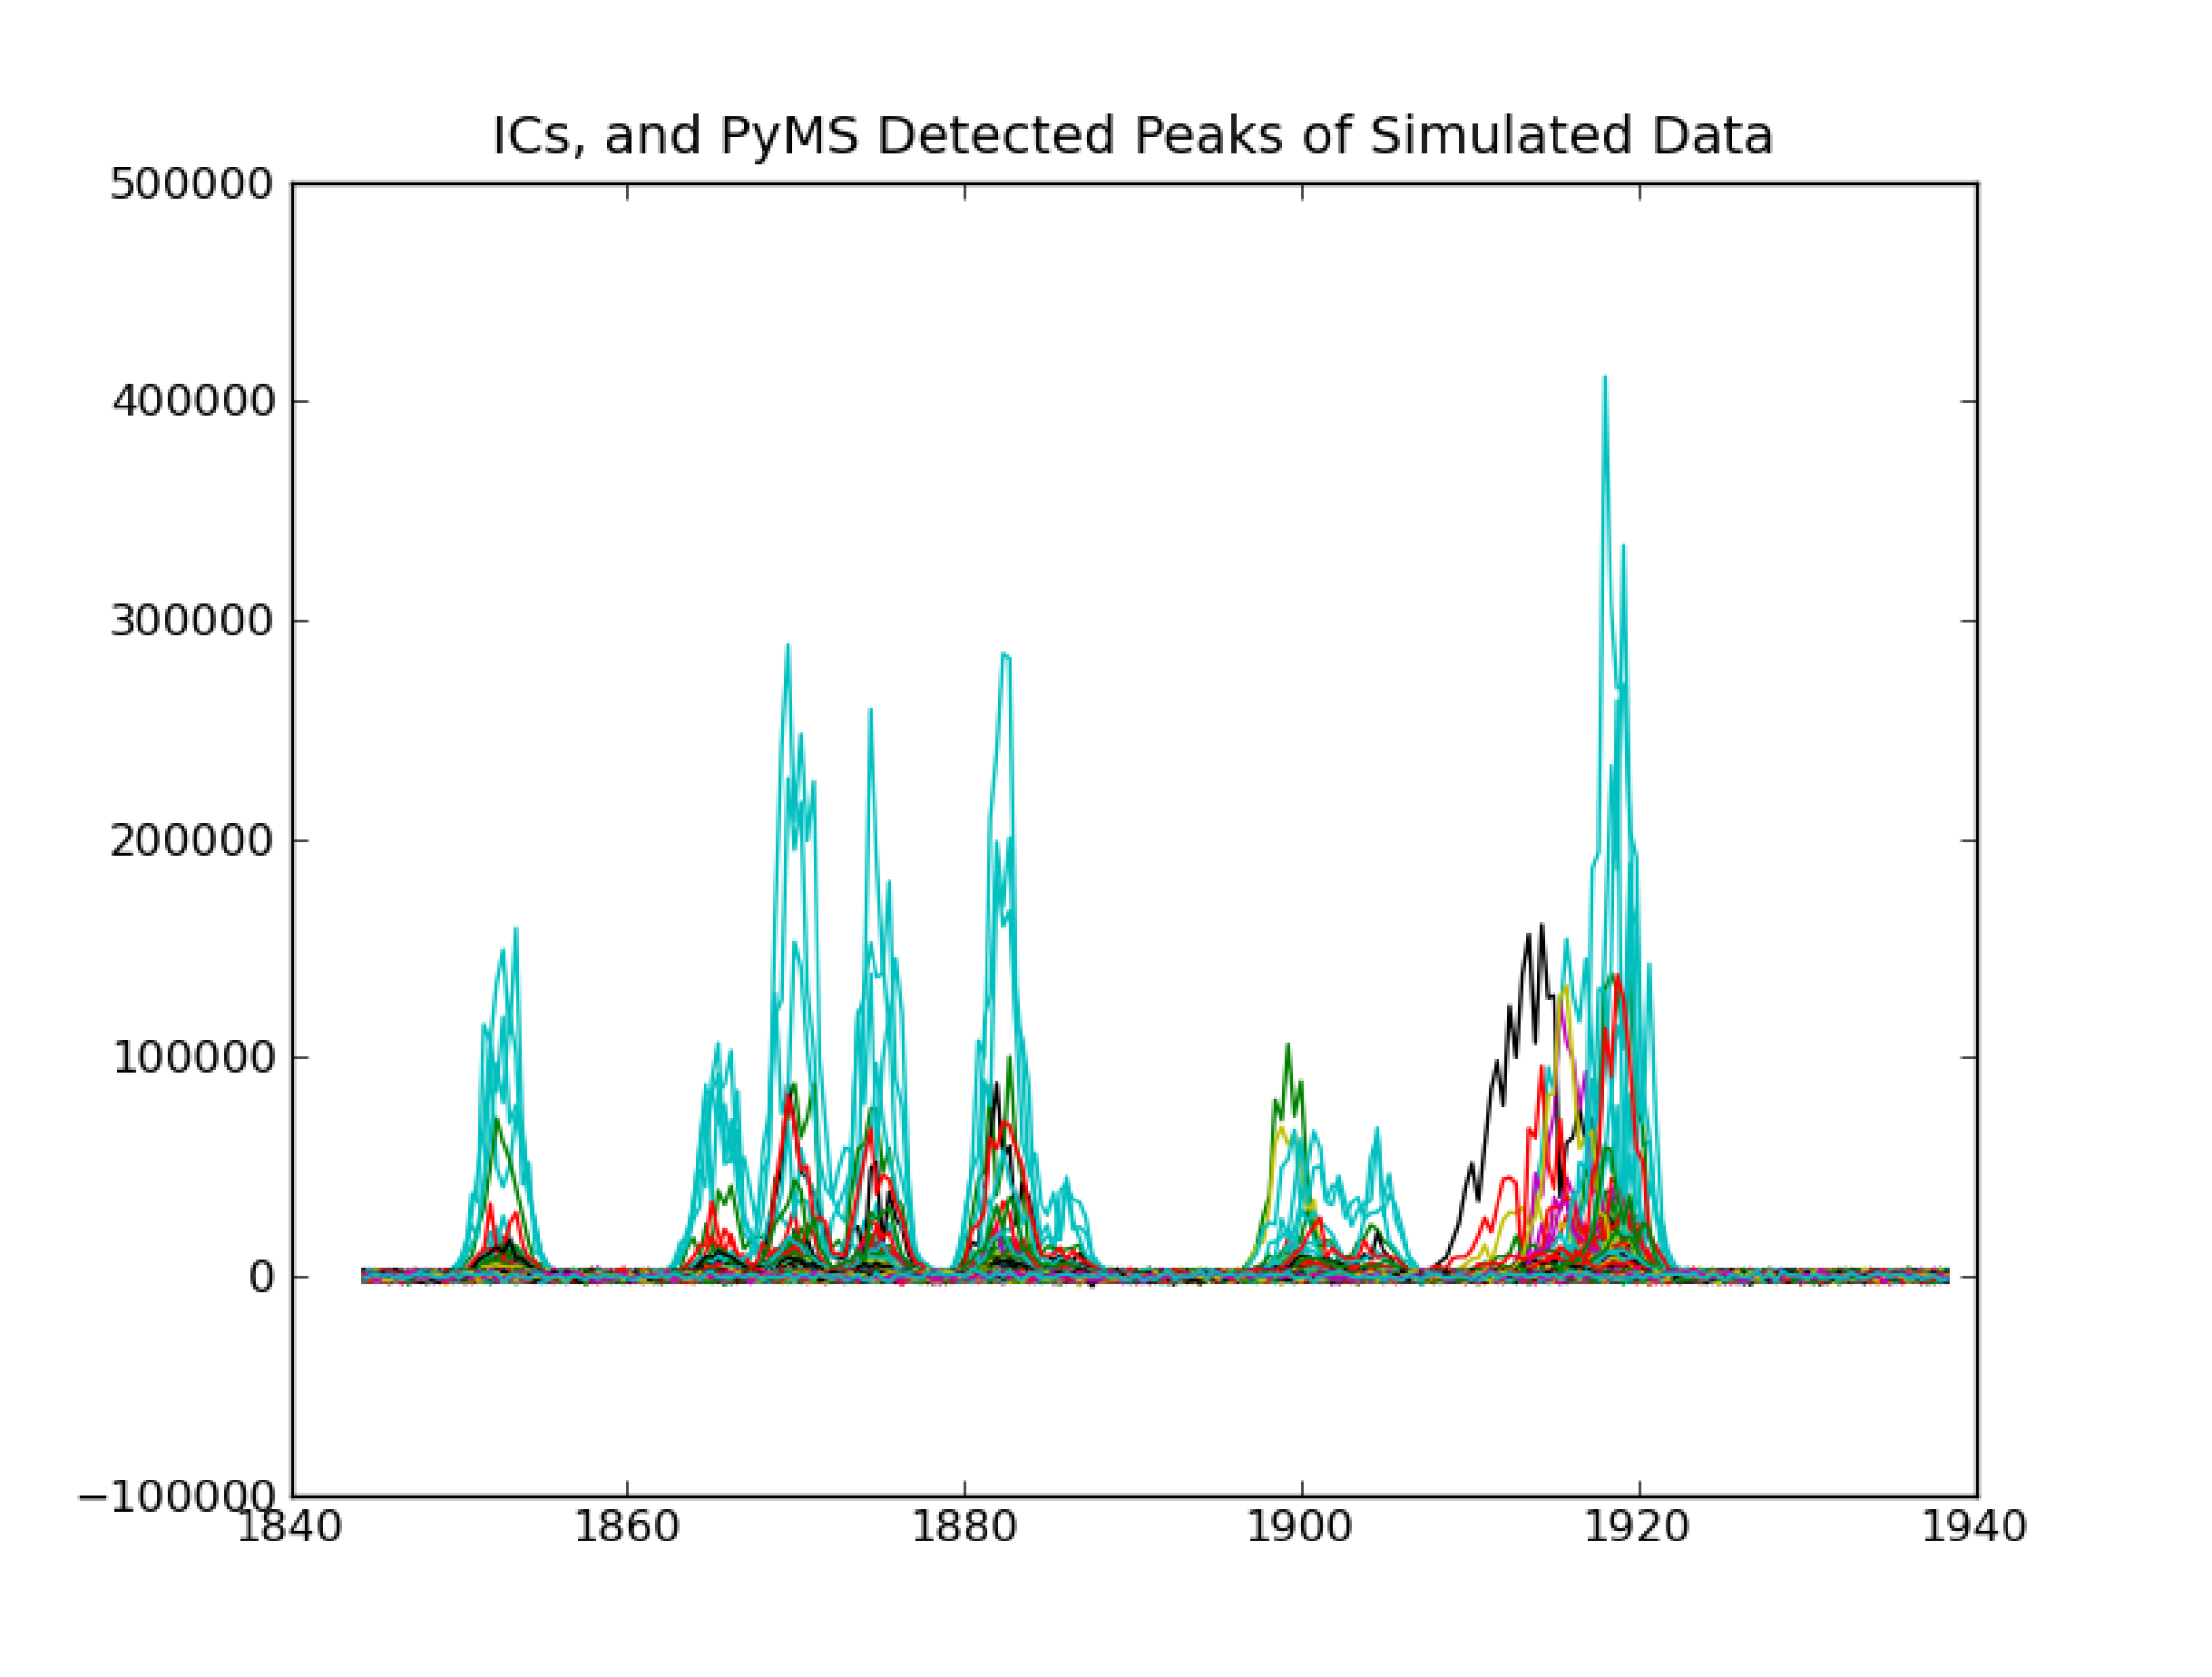
\includegraphics[scale=0.25]{graphics/chapter09/test-94.eps}
  \end{center}
  \caption{Graphics window displayed by the script 94/proc.py}
  \label{fig:gaussv-noise}
\end{figure}

\section{Detecting Peaks in the Simulated data}

\noindent
[ {\em This example is in pyms-test/95} ]

The simulated intensity matrix may be processed in PyMS in the same way as an intensity
matrix derived from real data. Applying the same techniques as outlined in section 
\ref{sec:peak-detection}, the peaks of the simulated IM with added noise from 
\ref{subsec:gaussv-noise} above can be found and displayed.

The found peaks are shown below in fig \ref{fig:sim-peaks}.

\begin{figure}[h]
  \begin{center}
    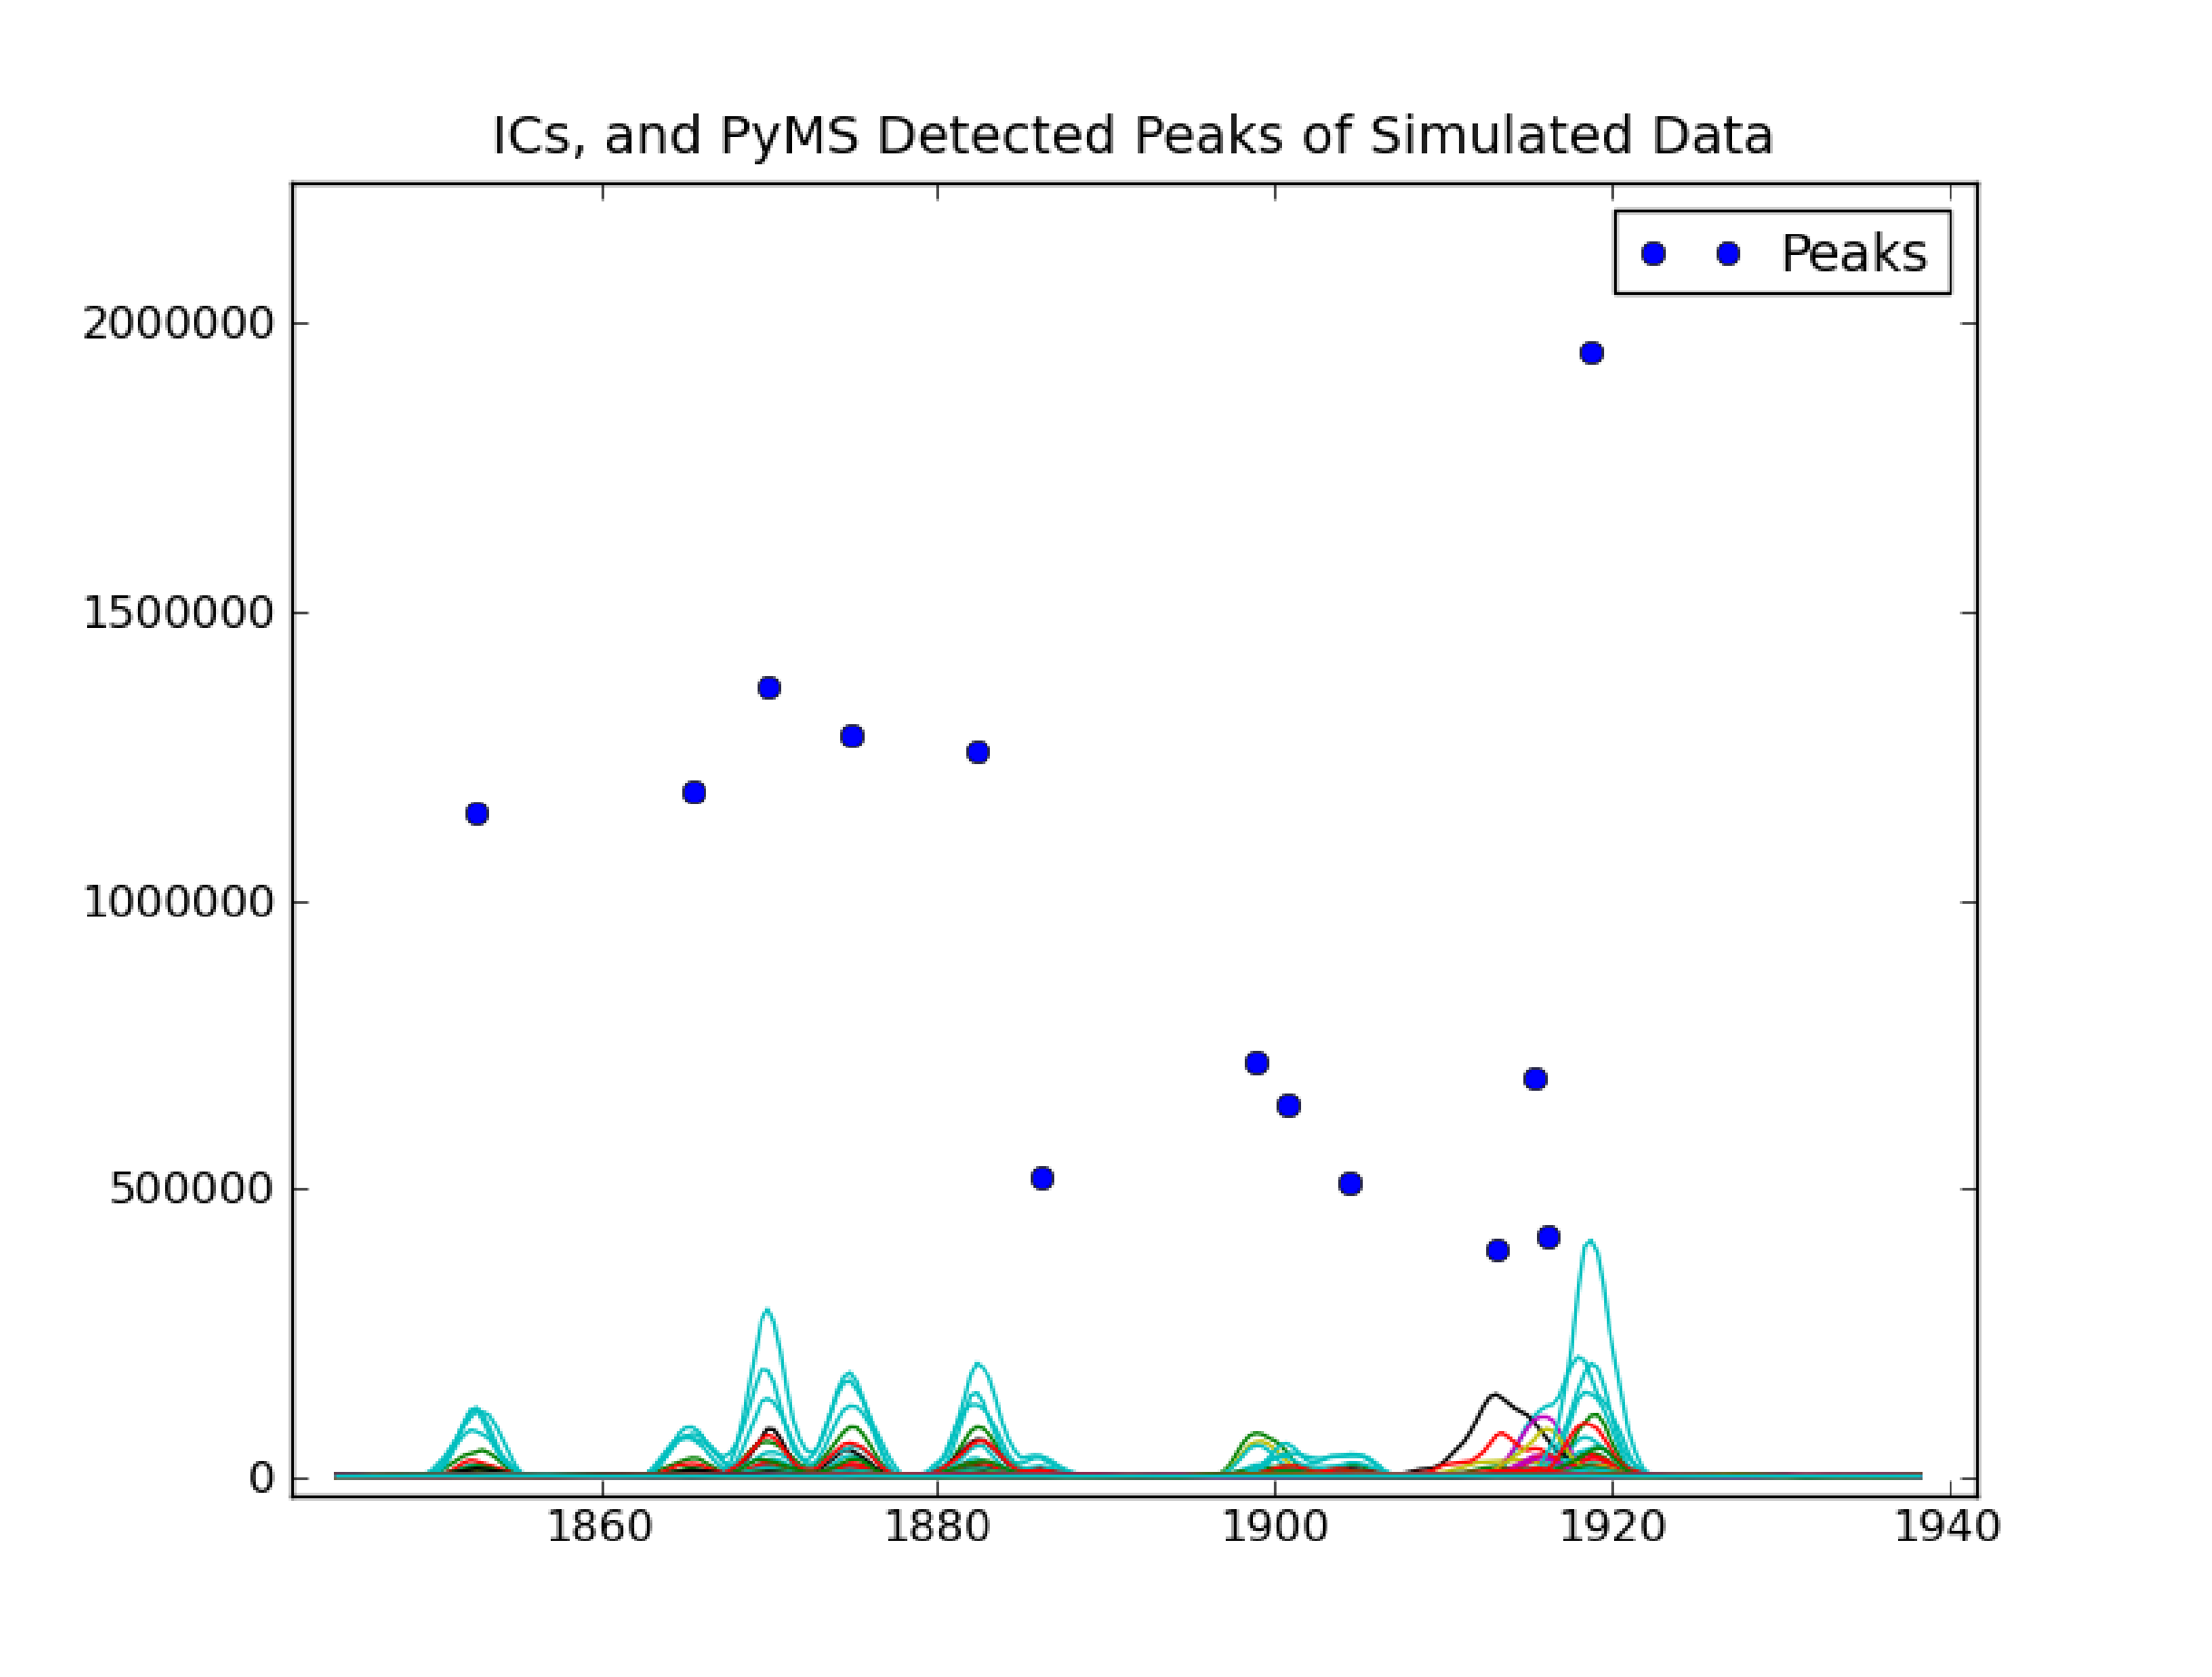
\includegraphics[scale=0.25]{graphics/chapter09/test-95.eps}
  \end{center}
  \caption{Graphics window displayed by the script 95/proc.py}
  \label{fig:sim-peaks}
\end{figure}
